\chapter{Simulations}
\label{ch:results}

\section{Performance Metrics}
In this section, we will introduce three performance metrics that are often used to measure the quality of reconstructed images and videos.

Let $\bm \hat{v} \in\mathbb{R}^M$ be a reconstructed signal (in vectorized form) and let $\bm v$ be the corresponding orginal signal.
The \emph{mean square error} (MSE) of the reconstruction is defined as
\begin{equation*}
  \mse(\bm{\hat v}) = \frac{\sum_{i=1}^M (\hat v_i - v_i)^2}{M}
\end{equation*}
The MSE is zero if and only if we $\bm{\hat v}$ is an exact reconstruction of $\bm v$.

Using the MSE, we can compute the \emph{Peak Signal-to-Noise Ratio} (PSNR) of the reconstruction:
\begin{equation*}
  \psnr(\bm{\hat v}) = 10 \cdot \log_{10} \left(\frac{R^2}{\mse(\bm{\hat v})}\right)
\end{equation*}
where $R$ is the maximum fluctuation in the input signal data type. 
For grayscale images or videos in which the pixel values are stored as 8-bit unsigned integers, we have that $R = 256$.

The PSNR is usually expressed in term of decibel (dB). 
Higher values of the PSNR correspond to more accurate reconstructions.
The PSNR is widely used in the image and video compression literature to measure the quality of a compressed signal.
Generally, when comparing the reconstruction quality, the PSNR should only be used if it was measured on the same signal.

The final performance metric that we compute is the \emph{relative reconstruction error}.
It is given by
\begin{equation*}
  \rre(\bm{\hat v}) = \frac{||\bm{\hat v} - \bm v||_2}{||\bm v||_2}
\end{equation*}
This is the metric that was used in \cite{ji2008} and \cite{pilikos2014}.


\section{Performance Evaluation}



\begin{figure}
  \centering
  \begin{tikzpicture}[scale = 0.8,baseline]
    \begin{axis}[
      xlabel=$N/M$ (\%),
      ylabel=$\rre$ (\%),
      xmin=0, xmax = 100,
      ymin = 0, 
      scaled ticks=false,
      yticklabel style={
        /pgf/number format/precision=2,
        /pgf/number format/fixed,
      }
      ]
      \addplot table [x=pc, y=rre] {Chapter7/Images/MSCE.dat};      
    \end{axis}
  \end{tikzpicture}
  % 
  \hskip 10pt
  % 
  \begin{tikzpicture}[scale = 0.8,baseline]
    \begin{axis}[
      xlabel=$N/M$ (\%),
      ylabel=$\psnr$,
      xmin=0, xmax = 90,      
      scaled ticks=false,
      yticklabel style={
        /pgf/number format/precision=2,
        /pgf/number format/fixed,
      }
      ]
      \addplot table [x=pc, y=psnr] {Chapter7/Images/MSCE.dat};      
    \end{axis}
  \end{tikzpicture}
\caption{Performance of MSCE with 3 cascades and uniform Masks}
\end{figure}

\begin{figure}
  \centering
  \begin{tikzpicture}[scale = 0.8,baseline]
    \begin{axis}[
      xlabel=$N/M$ (\%),
      ylabel=$\rre$ (\%),
      xmin=0, xmax = 100,
      ymin = 0, 
      scaled ticks=false,
      yticklabel style={
        /pgf/number format/precision=2,
        /pgf/number format/fixed,
      }
      ]
      \addplot table [x=pc, y=rre] {Chapter7/Images/GAUSS_DCT.dat};      
      \addlegendentry{DCT}
      \addplot table [x=pc, y=rre] {Chapter7/Images/GAUSS_HAAR.dat};      
      \addlegendentry{Haar}
    \end{axis}
  \end{tikzpicture}
  % 
  \hskip 10pt
  % 
  \begin{tikzpicture}[scale = 0.8,baseline]
    \begin{axis}[
      xlabel=$N/M$ (\%),
      ylabel=$\psnr$,
      xmin=0, xmax = 90,      
      scaled ticks=false,
      legend style={
        at={(0.03,0.98)},
        anchor=north west,
      },
      yticklabel style={
        /pgf/number format/precision=2,
        /pgf/number format/fixed,
      }
      ]
      \addplot table [x=pc, y=psnr] {Chapter7/Images/GAUSS_DCT.dat};      
      \addlegendentry{DCT}
      \addplot table [x=pc, y=psnr] {Chapter7/Images/GAUSS_HAAR.dat};      
      \addlegendentry{Haar}
    \end{axis}
  \end{tikzpicture}
\caption{DCT vs Haar DWT (scale 3) with Gaussian measurements}
\end{figure}

\begin{figure}
  \centering
  \begin{tikzpicture}[scale = 0.8,baseline]
    \begin{axis}[
      xlabel=$N/M$ (\%),
      ylabel=$\rre$ (\%),
      xmin=0, xmax = 100,
      ymin = 0, 
      scaled ticks=false,
      yticklabel style={
        /pgf/number format/precision=2,
        /pgf/number format/fixed,
      }
      ]
      \addplot table [x=pc, y=rre] {Chapter7/Images/GAUSS_DCT.dat};      
      \addlegendentry{Gauss}
      \addplot table [x=pc, y=rre] {Chapter7/Images/BERN_DCT.dat};      
      \addlegendentry{Bernoulli}
      \addplot table [x=pc, y=rre] {Chapter7/Images/MASK_DCT.dat};      
      \addlegendentry{Mask}
    \end{axis}
  \end{tikzpicture}
  % 
  \hskip 10pt
  % 
  \begin{tikzpicture}[scale = 0.8,baseline]
    \begin{axis}[
      xlabel=$N/M$ (\%),
      ylabel=$\psnr$,
      xmin=0, xmax = 90,      
      scaled ticks=false,
      legend style={
        at={(0.03,0.98)},
        anchor=north west,
      },
      yticklabel style={
        /pgf/number format/precision=2,
        /pgf/number format/fixed,
      }
      ]
      \addplot table [x=pc, y=psnr] {Chapter7/Images/GAUSS_DCT.dat};      
      \addlegendentry{Gauss}
      \addplot table [x=pc, y=psnr] {Chapter7/Images/BERN_DCT.dat};      
      \addlegendentry{Bernoulli}
      \addplot table [x=pc, y=psnr] {Chapter7/Images/MASK_DCT.dat};      
      \addlegendentry{Mask}
    \end{axis}
  \end{tikzpicture}
\caption{Gaussian vs Bernoulli vs Mask (uniform) with DCT basis}
\end{figure}

%% SCALES
\begin{figure}
  \centering
  \begin{tikzpicture}[scale = 0.8,baseline]
    \begin{axis}[
      xlabel=$N/M$ (\%),
      ylabel=$\rre$ (\%),
      xmin=0, xmax = 100,
      ymin = 0, 
      scaled ticks=false,
      yticklabel style={
        /pgf/number format/precision=2,
        /pgf/number format/fixed,
      }
      ]
      \addplot table [x=pc, y=rre] {Chapter7/Images/HAAR_GAUSS_1.dat};      
      \addlegendentry{Scale 1}
      \addplot table [x=pc, y=rre] {Chapter7/Images/HAAR_GAUSS_2.dat};
      \addlegendentry{Scale 2}
      \addplot table [x=pc, y=rre] {Chapter7/Images/HAAR_GAUSS_3.dat};
      \addlegendentry{Scale 3}
    \end{axis}
  \end{tikzpicture}
  % 
  \hskip 10pt
  % 
  \begin{tikzpicture}[scale = 0.8,baseline]
    \begin{axis}[
      xlabel=$N/M$ (\%),
      ylabel=$\psnr$,
      xmin=0, xmax = 90,      
      scaled ticks=false,
      legend style={
        at={(0.03,0.98)},
        anchor=north west,
      },
      yticklabel style={
        /pgf/number format/precision=2,
        /pgf/number format/fixed,
      }
      ]
      \addplot table [x=pc, y=psnr] {Chapter7/Images/HAAR_GAUSS_1.dat};
      \addlegendentry{Scale 1}
      \addplot table [x=pc, y=psnr] {Chapter7/Images/HAAR_GAUSS_2.dat};
      \addlegendentry{Scale 2}
      \addplot table [x=pc, y=psnr] {Chapter7/Images/HAAR_GAUSS_3.dat};
      \addlegendentry{Scale 3}
    \end{axis}
  \end{tikzpicture}
\caption{Haar wavelets at different scales with Gaussian measurements (fixed block size)}
\end{figure}

\clearpage

\section{Example Results}

\begin{figure}[!ht]
  \centering
  \textbf{\hspace{0.2in} Frame 2 \hspace{1.5in} Frame 19\hspace{0.5in}\vspace{0.2in}}
  \begin{subfigure}{0.4\textwidth}
    \centering
    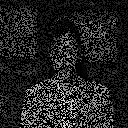
\includegraphics[width=0.8\textwidth]{Chapter7/Images/akiyo40_masked_2.png}
    \caption{Corrupted}
  \end{subfigure}
  \begin{subfigure}{0.4\textwidth}
    \centering
    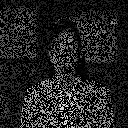
\includegraphics[width=0.8\textwidth]{Chapter7/Images/akiyo40_masked_19.png}
    \caption{Corrupted}
  \end{subfigure}
  \begin{subfigure}{0.4\textwidth}
    \centering
    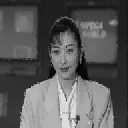
\includegraphics[width=0.8\textwidth]{Chapter7/Images/akiyo40_rec_2.png}
    \caption{Recovered}
  \end{subfigure}
  \begin{subfigure}{0.4\textwidth}
    \centering
    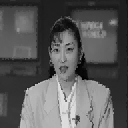
\includegraphics[width=0.8\textwidth]{Chapter7/Images/akiyo40_rec_19.png}
    \caption{Recovered}
  \end{subfigure}
  \begin{subfigure}{0.4\textwidth}
    \centering
    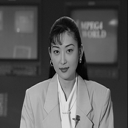
\includegraphics[width=0.8\textwidth]{Chapter7/Images/akiyo40_orig_2.png}
    \caption{Original}
  \end{subfigure}
  \begin{subfigure}{0.4\textwidth}
    \centering
    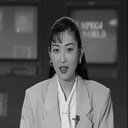
\includegraphics[width=0.8\textwidth]{Chapter7/Images/akiyo40_orig_19.png}
    \caption{Original}
  \end{subfigure}
  \caption{Reconstruction of $128\times 128\times 128$ video signal ``akiyo'' from 40\% of the measurement using the MSCE with 3 cascades. Mask decimation pattern is uniform. $\psnr = 30.02$}
\end{figure}

\begin{figure}
  \centering
  \textbf{\hspace{0.2in} Frame 32 \hspace{1.5in} Frame 52\hspace{0.5in}\vspace{0.1in}}
  \begin{subfigure}{0.4\textwidth}
    \centering
    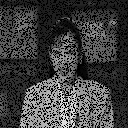
\includegraphics[width=0.9\textwidth]{Chapter7/Images/akiyo70_masked_32.png}
    \caption{Corrupted}
  \end{subfigure}
  \begin{subfigure}{0.4\textwidth}
    \centering
    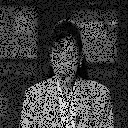
\includegraphics[width=0.9\textwidth]{Chapter7/Images/akiyo70_masked_52.png}
    \caption{Corrupted}
  \end{subfigure}
  \begin{subfigure}{0.4\textwidth}
    \centering
    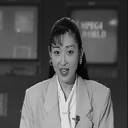
\includegraphics[width=.9\textwidth]{Chapter7/Images/akiyo70_rec_32.png}
    \caption{Recovered}
  \end{subfigure}
  \begin{subfigure}{0.4\textwidth}
    \centering
    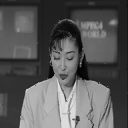
\includegraphics[width=.9\textwidth]{Chapter7/Images/akiyo70_rec_52.png}
    \caption{Recovered}
  \end{subfigure}
  \begin{subfigure}{0.4\textwidth}
    \centering
    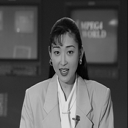
\includegraphics[width=.9\textwidth]{Chapter7/Images/akiyo70_orig_32.png}
    \caption{Original}
  \end{subfigure}
  \begin{subfigure}{0.4\textwidth}
    \centering
    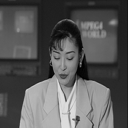
\includegraphics[width=.9\textwidth]{Chapter7/Images/akiyo70_orig_52.png}
    \caption{Original}
  \end{subfigure}
  \caption{Reconstruction of $128\times 128\times 128$ video signal ``akiyo'' from 70\% of the measurement using the MSCE with 3 cascades. Mask decimation pattern is uniform. $\psnr = 36.86$}
\end{figure}

\begin{figure}
  \centering
  \textbf{\hspace{0.2in} Frame 18 \hspace{1.5in} Frame 22\hspace{0.5in}\vspace{0.1in}}
  \begin{subfigure}{0.4\textwidth}
    \centering
    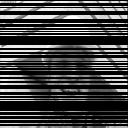
\includegraphics[width=.9\textwidth]{Chapter7/Images/foreman40_masked_18.png}
    \caption{Corrupted}
  \end{subfigure}
  \begin{subfigure}{0.4\textwidth}
    \centering
    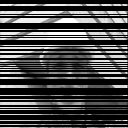
\includegraphics[width=.9\textwidth]{Chapter7/Images/foreman40_masked_22.png}
    \caption{Corrupted}
  \end{subfigure}
  \begin{subfigure}{0.4\textwidth}
    \centering
    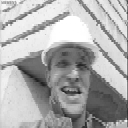
\includegraphics[width=.9\textwidth]{Chapter7/Images/foreman40_rec_18.png}
    \caption{Recovered}
  \end{subfigure}
  \begin{subfigure}{0.4\textwidth}
    \centering
    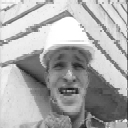
\includegraphics[width=.9\textwidth]{Chapter7/Images/foreman40_rec_22.png}
    \caption{Recovered}
  \end{subfigure}
  \begin{subfigure}{0.4\textwidth}
    \centering
    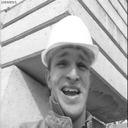
\includegraphics[width=.9\textwidth]{Chapter7/Images/foreman40_orig_18.png}
    \caption{Original}
  \end{subfigure}
  \begin{subfigure}{0.4\textwidth}
    \centering
    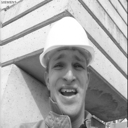
\includegraphics[width=.9\textwidth]{Chapter7/Images/foreman40_orig_22.png}
    \caption{Original}
  \end{subfigure}
  \caption{Reconstruction of $128\times 128\times 128$ video signal ``foreman'' from 40\% of the measurement using the MSCE with 3 cascades. Mask decimation pattern is: horizontal lines that are randomly generated for each frame. $\psnr = 25.50$}
\end{figure}


\begin{figure}
  \centering
  \textbf{\hspace{0.2in} Frame 18 \hspace{1.5in} Frame 22\hspace{0.5in}\vspace{0.1in}}
  \begin{subfigure}{0.4\textwidth}
    \centering
    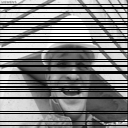
\includegraphics[width=.9\textwidth]{Chapter7/Images/foreman70_masked_18.png}
    \caption{Corrupted}
  \end{subfigure}
  \begin{subfigure}{0.4\textwidth}
    \centering
    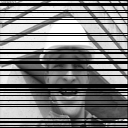
\includegraphics[width=.9\textwidth]{Chapter7/Images/foreman70_masked_22.png}
    \caption{Corrupted}
  \end{subfigure}
  \begin{subfigure}{0.4\textwidth}
    \centering
    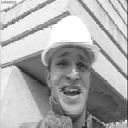
\includegraphics[width=.9\textwidth]{Chapter7/Images/foreman70_rec_18.png}
    \caption{Recovered}
  \end{subfigure}
  \begin{subfigure}{0.4\textwidth}
    \centering
    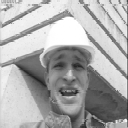
\includegraphics[width=.9\textwidth]{Chapter7/Images/foreman70_rec_22.png}
    \caption{Recovered}
  \end{subfigure}
  \begin{subfigure}{0.4\textwidth}
    \centering
    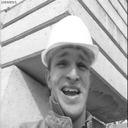
\includegraphics[width=.9\textwidth]{Chapter7/Images/foreman70_orig_18.png}
    \caption{Original}
  \end{subfigure}
  \begin{subfigure}{0.4\textwidth}
    \centering
    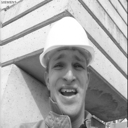
\includegraphics[width=.9\textwidth]{Chapter7/Images/foreman70_orig_22.png}
    \caption{Original}
  \end{subfigure}
  \caption{Reconstruction of $128\times 128\times 128$ video signal ``foreman'' from 70\% of the measurement using the MSCE with 3 cascades. Mask decimation pattern is: horizontal lines that are randomly generated for each frame. $\psnr = 30.32$}
\end{figure}

\begin{figure}
  \centering
  \textbf{\hspace{0.2in} Frame 11 \hspace{1.5in} Frame 12\hspace{0.5in}\vspace{0.1in}}
  \begin{subfigure}{0.4\textwidth}
    \centering
    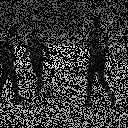
\includegraphics[width=.9\textwidth]{Chapter7/Images/soccer40_masked_11.png}
    \caption{Corrupted}
  \end{subfigure}
  \begin{subfigure}{0.4\textwidth}
    \centering
    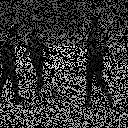
\includegraphics[width=.9\textwidth]{Chapter7/Images/soccer40_masked_12.png}
    \caption{Corrupted}
  \end{subfigure}
  \begin{subfigure}{0.4\textwidth}
    \centering
    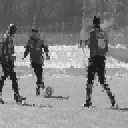
\includegraphics[width=.9\textwidth]{Chapter7/Images/soccer40_rec_11.png}
    \caption{Recovered}
  \end{subfigure}
  \begin{subfigure}{0.4\textwidth}
    \centering
    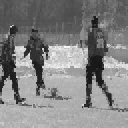
\includegraphics[width=.9\textwidth]{Chapter7/Images/soccer40_rec_12.png}
    \caption{Recovered}
  \end{subfigure}
  \begin{subfigure}{0.4\textwidth}
    \centering
    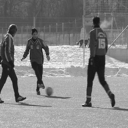
\includegraphics[width=.9\textwidth]{Chapter7/Images/soccer40_orig_11.png}
    \caption{Original}
  \end{subfigure}
  \begin{subfigure}{0.4\textwidth}
    \centering
    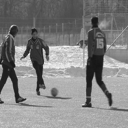
\includegraphics[width=.9\textwidth]{Chapter7/Images/soccer40_orig_12.png}
    \caption{Original}
  \end{subfigure}
  \caption{Reconstruction of $128\times 128\times 128$ video signal ``soccer'' from 40\% of the measurement using the MSCE with 3 cascades. Mask decimation pattern is: missing pixels that are constant across the frames. $\psnr = 24.84$}
\end{figure}



\begin{figure}
  \centering
  \textbf{\hspace{0.2in} Frame 11 \hspace{1.5in} Frame 12\hspace{0.5in}\vspace{0.1in}}
  \begin{subfigure}{0.4\textwidth}
    \centering
    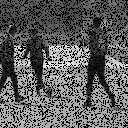
\includegraphics[width=.9\textwidth]{Chapter7/Images/soccer70_masked_11.png}
    \caption{Corrupted}
  \end{subfigure}
  \begin{subfigure}{0.4\textwidth}
    \centering
    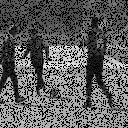
\includegraphics[width=.9\textwidth]{Chapter7/Images/soccer70_masked_12.png}
    \caption{Corrupted}
  \end{subfigure}
  \begin{subfigure}{0.4\textwidth}
    \centering
    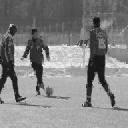
\includegraphics[width=.9\textwidth]{Chapter7/Images/soccer70_rec_11.png}
    \caption{Recovered}
  \end{subfigure}
  \begin{subfigure}{0.4\textwidth}
    \centering
    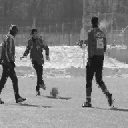
\includegraphics[width=.9\textwidth]{Chapter7/Images/soccer70_rec_12.png}
    \caption{Recovered}
  \end{subfigure}
  \begin{subfigure}{0.4\textwidth}
    \centering
    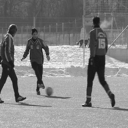
\includegraphics[width=.9\textwidth]{Chapter7/Images/soccer70_orig_11.png}
    \caption{Original}
  \end{subfigure}
  \begin{subfigure}{0.4\textwidth}
    \centering
    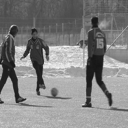
\includegraphics[width=.9\textwidth]{Chapter7/Images/soccer70_orig_12.png}
    \caption{Original}
  \end{subfigure}
  \caption{Reconstruction of $128\times 128\times 128$ video signal ``soccer'' from 70\% of the measurement using the MSCE with 3 cascades. Mask decimation pattern is: missing pixels that are constant across the frames. $\psnr = 29.35$}
\end{figure}

\begin{figure}
  \centering
  \textbf{\hspace{0.5in} Frame 21 \hspace{1.5in} Frame 151\hspace{0.5in}\vspace{0.2in}}
  \begin{subfigure}{0.4\textwidth}
    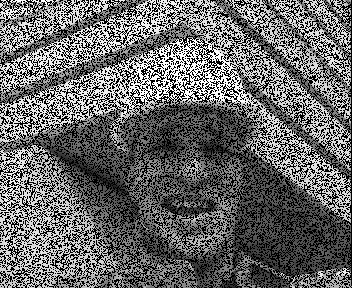
\includegraphics[width=\textwidth]{Chapter5/Images/foreman_masked_21.png}
    \caption{Corrupted}
  \end{subfigure}
  \begin{subfigure}{0.4\textwidth}
    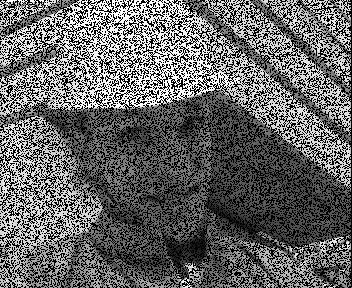
\includegraphics[width=\textwidth]{Chapter5/Images/foreman_masked_151.png}
    \caption{Corrupted}
  \end{subfigure}
  \begin{subfigure}{0.4\textwidth}
    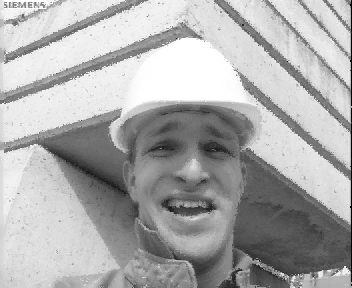
\includegraphics[width=\textwidth]{Chapter5/Images/foreman_rec_21.png}
    \caption{Recovered}
  \end{subfigure}
  \begin{subfigure}{0.4\textwidth}
    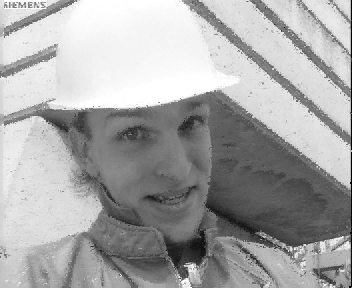
\includegraphics[width=\textwidth]{Chapter5/Images/foreman_rec_151.png}
    \caption{Recovered}
  \end{subfigure}
  \begin{subfigure}{0.4\textwidth}
    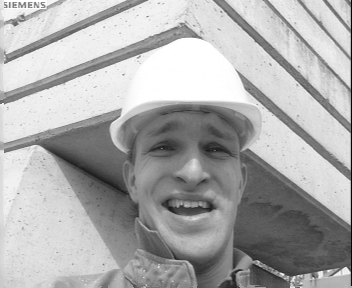
\includegraphics[width=\textwidth]{Chapter5/Images/foreman_orig_21.png}
    \caption{Original}
  \end{subfigure}
  \begin{subfigure}{0.4\textwidth}
    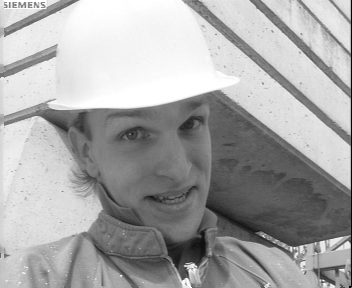
\includegraphics[width=\textwidth]{Chapter5/Images/foreman_orig_151.png}
    \caption{Original}
  \end{subfigure}
  \caption[Example output of our video interpolator]{Example of a masked video signal, where only 60\% of the pixel values are known (a-b). 
    Reconstruction via the MSCE Algorithm using 2 cascades (PSNR: 28.6) (c-d).
    Original video (e-f).}
  \label{fig:foreman_masked}
\end{figure}
